Photons are not just particles but also propagating waves. It is, however, very convenient to think of photons as just particles occupying states in the harmonic oscillator when describing interactions between photons and emitter systems such as atoms, quantum dots, or NV centers. Such a description is also sufficient when you deal with cavity quantum electrodynamics, where photons occupy localized cavity modes, and the Jaynes-Cummings model describes the interaction. The wave-like nature of the photon then enters the picture through the light-matter coupling given by the overlap between the local density of states and the dipole moment of the emitter \cite{Lodahl2015InterfacingNanostructuresb}. If the photon, however, is propagating in, e.g., a waveguide, such a simplification can no longer be made since the photon occupies a continuum of modes. It is now relevant to know "when" the photon arrives or, equivalently, which frequencies it contains. In this chapter, we introduce the theory of traveling quantum states of light using the photon time binning method of continuous fock states \cite{Heuck2020Photon-photonCavities}.  

\begin{figure}[H]
    \centering
    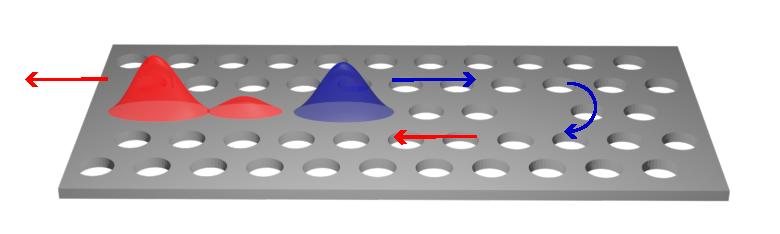
\includegraphics[width=\linewidth]{figures/onesided_cavity.pdf}
    \caption{Schematic of a photonic crystal waveguide containing an L1 cavity (one missing hole) interacting with an incoming (blue) pulse producing a scattered (red) pulse.}
    \label{fig:onesided_wg}
\end{figure}

\section{Continuous Fock States}
We can describe the traveling quantum pulse as occupying a collection of bosonic modes. As an example, a traveling single photon can be defined as \cite{Ciccarello2018CollisionOptics}:
\begin{equation}
    |\psi\rangle=\int \mathrm{d} \nu \psi(\nu) w^{\dagger}(\nu)| \emptyset \rangle,
\end{equation}
where $w^{\dagger}(\nu)$ is the creation operator for a photon of frequency $\nu$ with units of $\sqrt{\mathrm{time}}$ and $\psi(\nu)$ defines the wavefunction of the pulse also with units of $\sqrt{\mathrm{time}}$. The field operators $w(\nu)$ and $w^\dagger(\nu)$ obey the commutator relations: $\comm{w(\nu)}{w^\dagger(\nu ')} = \delta(\nu - \nu ')$, $\comm{w(\nu)}{w(\nu ')} = 0$, and $\comm{w^\dagger(\nu)}{w^\dagger(\nu ')} = 0$. The free evolution of the pulse is given by the Hamiltonian:

\begin{equation}
    H_f= \hbar \int \mathrm{d} \nu \nu w^{\dagger}(\nu) w(\nu)
\end{equation}

If we consider some cavity or emitter system with annihilation and creation operators $a$ and $a^\dagger$ (note that a two-level system is equivalent to a cavity with a cutoff of one photon and a more appropriate symbol would here be $\sigma$), the interaction $H_{int}$ with the pulse is, under the assumption of the Rotating Wave Approximation, given as \cite{Ciccarello2018CollisionOptics}:

\begin{equation}
    H_{int} = \hbar \int \mathrm{d} \nu  \left(g(\nu) a^{\dagger} w(\nu) + g(\nu)^{*} a w^{\dagger}(\nu)\right)
\end{equation}
where $g(\nu)$ defines the coupling strength with each individual mode in the pulse. If we transform into an interaction picture with respect to $H_f$ we get (see appendix \ref{app:rotating}):

\begin{equation}
    \mathrm{e}^{i H_f t /\hbar} H_{int} \mathrm{e}^{-i H_f t /\hbar} = H_{int}(t) =  \hbar \int \mathrm{d} \nu \left(g(\nu) a^{\dagger} w(\nu) \mathrm{e}^{i\nu t} + g(\nu)^{*} a w^{\dagger}(\nu) \mathrm{e}^{-i\nu t}\right)
\end{equation}

Assuming that the interaction $g(\nu)$ is spectrally flat $g(\nu) = i \sqrt{\gamma/2 \pi}$, we can make a considerable simplification of the above interaction by introducing the Fourier transformed field operator: $w(t)=\frac{1}{\sqrt{2 \pi}} \int \mathrm{d} \nu w(\nu) e^{-i \nu t}$ with units of $1/\sqrt{\mathrm{time}}$. Note that the imaginary part in the coupling $g(\nu)$ is just one definition and that it is equally valid to define it as $g(\nu) = \sqrt{\gamma/2 \pi}$. Inserting $g(\nu) = i \sqrt{\gamma/2 \pi}$, we get:
\begin{equation}
    H_{int}(t) =  \hbar i \sqrt{\gamma} (a^\dagger w(t)-a w^\dagger(t) ) \label{eq:interaction}
\end{equation}
The implication of the above simplification is clear: the interaction is now only with a single (time) mode $w(t)$ at each time $t$. The single photon state can equivalently be defined as:

\begin{equation}
    \ket{\psi} = W^\dagger[\xi] \ket{\emptyset} = \int_{t_0}^{t_{end}} \mathrm{d}t \ \xi^{(1)}(t) w^\dagger(t) \ket{\emptyset} \label{eq:singlephoton}
\end{equation}
here $W^\dagger(\xi)$ creates a photon with the wavefunction $\xi^{(1)}(t)$ and by insertion we can show that $\xi^{(1)}(t) = \frac{1}{\sqrt{2 \pi}} \int \mathrm{d} \nu \psi(\nu) e^{-i \nu t} $. Here, $w^\dagger(t)$ is the creation operator for a photon at time $t$. The inner product $\bra{\psi} w^\dagger(t) w(t) \ket{\psi} = |\xi^{(1)}(t)|^2$ with units of inverse time thus gives the flux of photons at time $t$ and multiplied with a small timestep $\Delta t |\xi^{(1)}(t)|^2$ the probability of observing a photon at time $t$. 

We can take this picture of only interacting with a single mode at a time further and discretize the continuous fock state into time bins of width $\Delta t$. This amounts to defining new discretized annihilation and creation operators as \cite{Heuck2020Photon-photonCavities} (see also appendix \ref{app:rotating}):
\begin{equation}
     w(t_k) = w(k \Delta t) \rightarrow  \frac{w_k}{\sqrt{\Delta t}} \ \ \  \text{with} \ \comm{w_j}{w_k^\dagger} = \delta_{jk}
\end{equation}
where $w_k$ is the descritized (unitless) operator of the $k$th timebin and the factor of $1/\sqrt{\Delta t}$ assures the commutator relation in the limit of $\Delta t \rightarrow 0$. This means that the single photon continuous fock state becomes:
\begin{equation}
    \ket{\psi} = \int_{t_0}^{t_{end}} \mathrm{d}t \ \xi^{(1)}(t) w^\dagger(t) \ket{\emptyset}  \rightarrow 
\sum_{k=1}^N \sqrt{\Delta t} \xi(t_k) w_k^\dagger \ket{\emptyset} = \sum_{k=1}^N \sqrt{\Delta t} \xi(t_k) \ket{1_k} 
\end{equation}
where we introduced the binned photon state: $\ket{1_k}  = w_k^\dagger \ket{\emptyset}$. We now see that: $\bra{\psi} w_{k}^\dagger w_k \ket{\psi} = \Delta t \abs{\xi(t_k)}^2$ and the annihilation and creation operators $w_k$ and $w_k^\dagger$  now describes the probability of observing a photon in time bin $k$.
%The assumption of the interaction with the emitter/cavity being $g(\nu) = \sqrt{\gamma/2 \pi}$ can now also be motivated from a physical perspective. We expect the picture of only interacting with a single time-bin at a time to be valid if the field does not change significantly over the emitter/cavity. This is also known as the dipole approximation.

The interaction Hamiltonian equivalently becomes:
\begin{equation}
    H_{int}(t) =  \sum_k f_k(t) H_{k,int} = \sum_k f_k(t) i \hbar \sqrt{\gamma/\Delta t} (a^\dagger w_k - a w_k^\dagger) \label{eq:discretized_interaction}
\end{equation}
where we defined:
\begin{equation}
f_k(t) = \begin{cases}
          1, & \text{if } t_k < t <t_k+\Delta t  \\
          0, & \text{otherwise}
\end{cases} = \Theta(t - t_k) - \Theta(t - (t_k + \Delta t)) \label{eq:fk}    
\end{equation}
where $\Theta$ is the heaviside function and $H_{k,int} = i \hbar \sqrt{\gamma/\Delta t} (a^\dagger w_k - a w_k^\dagger)$. The Hamiltonian is thus constant within each time-bin, which reduces the numerical complexity significantly. It also allows for an intuitive mental picture: We are moving a conveyor belt of photon bins and letting one bin of the belt interact with the system at a time. This is also illustrated in Fig.~\ref{fig:conveyor}. Throughout the thesis, we will use the subscript $k$ on a Hamiltonian $H_k$ to denote that it follows the form in \eqref{eq:discretized_interaction}, and it is thus understood that the Hamiltonian is changing with each timestep $k$, but is constant WITHIN each timestep.

\begin{figure}
    \centering
    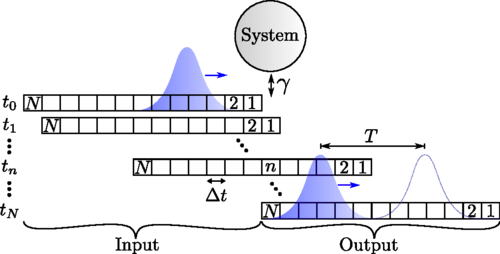
\includegraphics[width = 0.5 \linewidth]{figures/medium (1).png}
    \caption{Illustration of the interaction with one part of the pulse at a time. In the top row, an initial continuous fockstate is divided across N bins. At the subsequent timesteps labeled $t_i$, bin number $i$ interacts with the system. Once all bins have interacted with the system, the state in the bins is the output state. Image taken from ref. \cite{Heuck2020Photon-photonCavities}}
    \label{fig:conveyor}
\end{figure}


\section{Scattering on Onesided Cavity \label{sec:onephoton_scat}}
In the previous section, we introduced the time-bin formalism, and in this section, we are going to use it to derive the dynamics of a single photon pulse scattering on a single-sided cavity. Such a system can also be seen in Fig.~\ref{fig:onesided_wg}, where a photonic crystal waveguide carries a quantum pulse that interacts with a one-sided cavity. The differential equations governing the dynamics are defined from the Hamiltonian in eq.~\ref{eq:discretized_interaction}. Since the Hamiltonian is constant within each time-bin, we can describe the evolution from time-bin $n-1$ to $n$ by the unitary evolution \cite{Heuck2020Photon-photonCavities}:
\begin{equation}
    U_n = U(t_{n-1},t_{n}) = \exp \left(- \int_{t_{n-1}}^{t_{n-1}+\Delta t} \frac{i}{\hbar} H_{int}(t^{\prime}) d t^{\prime} \right)  =\exp \left(-\frac{i}{\hbar} H_{k,int} \Delta t\right)=\sum_{m=0}^{\infty} \frac{1}{m !}\left(-\frac{i}{\hbar} H_{n,int} \Delta t\right)^m
\end{equation}
which thus relates the state at time $t_{n-1}$ to the state at time $t_n$ as: $U_n \ket{\psi_{n-1}} = \ket{\psi_n}$, where $\ket{\psi_k}$ denote the state at time $t_k$. Up to first order in $\Delta t$, $U_n$ is given as:
\begin{equation}
    U_n \approx 1+\sqrt{\gamma \Delta t}\left(a^{\dagger} w_n-a w_n^{\dagger}\right)-\frac{\gamma}{2} \Delta t a^{\dagger} a w_n w_n^{\dagger} \label{eq:unitaryevolution}
\end{equation}
We consider the initial state being zero photons in the cavity and a one photon wavepacket (we use the Ket $\ket{\emptyset}$ to describe the vacuum of the waveguide, whereas $\ket{0}$ to describe the vacuum of the cavity):
\begin{equation}
    \left|\psi_0\right\rangle = \sum_{k=1}^N \sqrt{\Delta t} \xi(t_k) \ket{0} \ket{1_k} \label{eq:initial_single}
\end{equation}
The updated state after the first interaction with the time-bin is then given as:
\begin{equation}
    \ket{\psi_1} = U_1 \ket{\psi_0} = \sum_{k=2}^N \sqrt{\Delta t} \xi(t_k) \ket{0} \ket{1_k} + \sqrt{\Delta t} \xi(t_1) \ket{0} \ket{\mathbf{1}_1} + \sqrt{\gamma}  \Delta t \xi(t_1) \ket{1}\ket{\emptyset}
\end{equation}
where we have introduced bold enumeration $\ket{\mathbf{1}_1}$ for the time-bins that have passed the cavity to make the bookkeeping easier. We also introduce $\psi_1(t_1) =\sqrt{\gamma}  \Delta t \xi(t_1)$ as the amplitude of the cavity excitation at time $t_1$. After step two, we then have:

\begin{equation}
\begin{aligned}
    \ket{\psi_2} = U_2 \ket{\psi_1} &= \sum_{k=3}^N \sqrt{\Delta t} \xi(t_k) \ket{0} \ket{1_k} + \sum_{k=1}^2 \sqrt{\Delta t} \xi(t_k) \ket{0} \ket{\mathbf{1}_k} - \sqrt{\gamma \Delta t} \psi_1(t_1) \ket{0}\ket{\mathbf{1}_2} \\
    & + \sqrt{\gamma}  \Delta t \xi(t_2) \ket{1}\ket{\emptyset} - \frac{\gamma}{2} \Delta t \psi(t_1) \ket{1}\ket{\emptyset} + \psi_1(t_1) \ket{1}\ket{\emptyset}
\end{aligned}
\end{equation}


We notice that we can collect the terms in front of the bins that have passed the cavity as $\xi_{out}(t_2) = \xi(t_2) - \sqrt{\gamma} \psi_1(t_1)$ and the amplitude of the cavity now reads: $\psi_1(t_2) = \psi_1(t_1) -\gamma/2 \Delta t \psi_1(t_1) + \sqrt{\gamma}\Delta t \xi(t_2)$. We can generalize these update rules as:
\begin{equation}
    \psi_1(t_{n+1}) = \psi_1(t_n) -\frac{\gamma}{2} \Delta t \psi_1(t_n) + \sqrt{\gamma}\Delta t \xi(t_{n+1}) \label{eq:updaterule} 
\end{equation}
\begin{equation}
    \xi_{out}(t_{n+1}) = \xi(t_{n+1}) - \sqrt{\gamma} \psi_1(t_{n}) 
\end{equation}
If we take the limit of $\Delta t \rightarrow 0$, we have $t_{n+1} = t_n$ and rearranging eq.~\ref{eq:updaterule}, we arrive at the differential equation:
\begin{equation}
    \frac{\psi_1(t_{n+1}) - \psi_1(t_n)}{\Delta t} \xrightarrow[]{\Delta t \rightarrow 0} \frac{d \psi_1(t)}{d t}  = -\frac{\gamma}{2} \psi_1(t) + \sqrt{\gamma} \xi^{(1)}(t)
\end{equation}
Solving the differential equation then gives access to the scattered or output field by the input-output relation $\xi_{out}(t) = \xi^{(1)}(t) - \sqrt{\gamma} \psi_1(t)$. 

In a more realistic case, we could add a detuning between the pulse and the cavity $\delta = \omega_{c} - \omega_{w}$, where $\omega_{c}$ is the cavity frequency and $\omega_{w}$ is the central frequency of the waveguide pulse. As shown in the appendix \ref{app:rotating}, moving into the rotating frame would correspond to adding the term $\delta a^\dagger a$ to the Hamiltonian in eq.~\eqref{eq:discretized_interaction}. To get the correct equations of motion, we would then have to rederive the above equations. Luckily, in the above case, the detuning term is simple and just adds a phase term $-i\delta \Delta t a^\dagger a$ to the unitary in eq.~\eqref{eq:unitaryevolution}, which in turn just adds a phase term in the equation of motion:
%Note that due to the pulse's finite temporal shape, it contains multiple frequencies. However, as shown in appendix \ref{app:rotating}, if one assumes cavity frequencies in the visible spectrum (THz) regime and pulse durations of around several $\mathrm{ps}$, then the frequency spread (GHz) is negligible. Thus, a
\begin{equation}
    \frac{d \psi_1(t)}{d t}  = -(i \delta_a +\frac{\gamma}{2}) \psi_1(t) + \sqrt{\gamma} \xi^{(1)}(t) \label{eq:single_EOM}
\end{equation}
One could, however, easily imagine that adding more complicated terms to the Hamiltonian would require a more cumbersome rederivation. Indeed, as we shall see in the next section, an initial state consisting of two photons leads to additional possible paths of a photon, resulting in significantly more complex equations of motion. Automating this process to be less tedious is one of the main motivations behind the numerical method introduced in Chapter \ref{ch3}.

\section{Two-photon Continuous Fockstates \label{sec:twophoton_continuous}}
Before we introduce our new numerical method, let us, however, get some intuition for traveling two-photon states and why they complicate the scattering. 
It is straightforward to extend the single-photon state defined in eq.~\eqref{eq:singlephoton} to a two-photon continuous state as \cite{Baragiola2012N-PhotonSystem}:

\begin{align}
\frac{1}{\sqrt{2}}\left[W^\dagger[\xi]\right]^2| \emptyset \rangle = \frac{1}{\sqrt{2}} \int_{t_0}^{t_{end}} d t^{\prime} \int_{t_0}^{t_{end}} d t \ \xi^{(2)}(t,t^{\prime}) w^\dagger(t) w^\dagger\left(t^{\prime}\right)|\emptyset \rangle  
\end{align}
where $\xi^{(2)}(t,t') = \xi^{(1)}(t)\xi^{(1)}(t')$ is the two-photon wavefunction. The state is now defined over two times, describing the probability of observing a photon at time $t$ and another at time $t'$. In this case, the two-photon wavefunction is a product state, and both probabilities are described by the same single-photon wavefunction $\xi^{(1)}(t)$. This will, in general, not be the case. However, one can always expand the two-photon wavefunction in terms of products of one-photon wavefunctions via a Singular Value Decomposition (SVD) as \cite{Yang2022DeterministicSystems}:
\begin{equation}
    \xi^{(2)}(t,t') = \sum_i \lambda_i \phi_i(t) \phi_i(t') \label{eq:SVD}
\end{equation}
where $\phi_i(t)$ are orthonormal basis functions and if we have a normalized wavefunction $\sum_i\lambda_i^2 = 1$. In the above product state, we would thus have $\lambda_1^2 = 1$, i.e., the two-photon wavefunction contains only a product state of two single-photon states. It is now also clear that the wavefunction fulfills $\xi^{(2)}(t,t') = \xi^{(2)}(t',t)$, as expected for bosons. When discretizing the photon into bins, we thus only need $\approx N^2/2$ bins. This can be seen by:
\begin{align}
\frac{1}{\sqrt{2}} \left[W^\dagger(\xi)\right]^2|\emptyset \rangle &= \frac{1}{\sqrt{2}} \int_{t_0}^{t_{end}} d t^{\prime} \int_{t_0}^{t_{end}} d t \ \xi^{(2)}(t,t^{\prime}) w^\dagger(t) w^\dagger\left(t^{\prime}\right)|\emptyset \rangle \\
& \rightarrow \frac{1}{\sqrt{2}} \sum_{i=1}^N \sum_{k=1}^N   \Delta t \xi^{(2)} \left (t_i,t_k\right ) w_i^\dagger w_k^{\dagger}|\emptyset\rangle \\
& = \frac{1}{\sqrt{2}} \sum_{i=1}^N \sum_{k \neq i}^N \Delta t \xi^{(2)} \left (t_i,t_k\right) w_i^{\dagger} w_k^{\dagger}|\emptyset\rangle + \frac{1}{\sqrt{2}} \sum_{i=1}^N \Delta t \xi^{(2)} \left (t_i,t_i\right )w_i^\dagger w_i^\dagger\left|\emptyset\right\rangle \\
& =\frac{2}{\sqrt{2}} \sum_{i=1}^N \sum_{k>i}^N \Delta t \xi^{(2)} \left (t_i,t_k\right )\left|1_{t_i} 1_{t_k}\right\rangle + \sum_{i=1}^N \Delta t \xi^{(2)} \left (t_i,t_i\right ) \left|2 t_i\right\rangle \\
& =\sqrt{2} \sum_{i=1}^N \sum_{k > i}^N \Delta t \xi^{(2)}\left (t_i,t_k\right ) \mid 1_{t_i} 1_{t_k}\rangle + \sum_{i=1}^N \Delta t \xi^{(2)}\left (t_i,t_i\right )\left|2 t_i\right\rangle
\end{align}
This will be important in the next chapter when we want to represent the state numerically. In deriving the equations of motion, we will be taking $\Delta t \rightarrow 0$ (and thus also $N \rightarrow \infty$), and the diagonal containing two photons in the same time-bin will be vanishingly small and can thus be omitted. This will not be the case in the numerical representation, but for now, we can take the initial state to be $\ket{\psi}_0 = \sqrt{2} \sum_{i=1}^N \sum_{k > i}^N \xi_2\left (t_i,t_k\right ) \ket{0} \ket{1_{i} 1_{k}} $. Applying the unitary operator in eq.~\eqref{eq:unitaryevolution} then leads to the following state after the first timestep:
\begin{equation}
    \ket{\psi_1} = U_1 \ket{\psi_0} = \ket{\psi_0} + \sqrt{2 \gamma \Delta t} \sum_k 
\xi(t_1,t_k) \Delta t \ket{1} \ket{\emptyset,1_k} = \ket{\psi_0} + \ket{\psi_{abs,1}}
\end{equation}
In the subsequent timestep, the complexity grows immediately as multiple processes can take place. We can break it into two scenarios; absorption of the next photon bin corresponding to $U_2 \ket{\psi}_0$ and evolution of the absorbed photon in the cavity  $U_2 \ket{\psi}_{abs,1}$:
\begin{equation}
    \ket{\psi_2} = U_2 \ket{\psi_1} =U_2 \ket{\psi_0} + U_2 \ket{\psi}_{abs,1}  
\end{equation}
The absorption of the next bin is simple:
\begin{equation}
    U_2 \ket{\psi_0} =  \ket{\psi_0} + \sqrt{2 \gamma \Delta t} \sum_k 
\xi(t_2,t_k) \Delta t \ket{1} \ket{\emptyset,1_k}
\end{equation}
whereas for the already absorbed photon, we have terms corresponding to the reemission of a photon, reflection of an input photon, and absorption of another photon:
\begin{align}
 U_2 \ket{\psi}_{abs,1} &= \ket{\psi}_{abs,1} +  \sqrt{2} \gamma \Delta t^2 \xi(t_1,t_2) \ket{2} \ket{\emptyset,\emptyset} - \sqrt{2} \gamma \Delta t \sum_k 
\xi(t_1,t_k) \Delta t \ket{0} \ket{\mathbf{1}_2,1_k}\\ &- \sqrt{2 \gamma \Delta t} \gamma \Delta t /2 \sum_{k \neq 2} 
\xi(t_1,t_k) \Delta t \ket{1} \ket{\emptyset,1_k} 
 - \sqrt{\gamma \Delta t} \gamma \Delta t \xi(t_1,t_2) \Delta t \ket{1} \ket{\emptyset,1_2} 
\end{align}
From here, it is easy to imagine the many branches appearing. A full derivation is not within the scope of this thesis. Instead, we state the results of previous derivations \cite{Korsgaard2021Few-PhotonThesis} leading to the equations of motion:

\begin{equation}
\begin{array}{lr}
\dot{\psi}_2\left(\tilde{t}_n\right)=\sqrt{2} \psi_1^{(2)}\left(\tilde{t}_n\right) \tilde{\xi}_{\text {in }}\left(\tilde{t}_n\right)-\psi_2\left(\tilde{t}_n\right)-2 i \tilde{\delta} \psi_2\left(\tilde{t}_n\right), & \psi_2(0)=0 \\
\dot{\psi}_1^{(2)}\left(\tilde{t}_n\right)=\sqrt{2} \tilde{\xi}_{\text {in }}\left(\tilde{t}_n\right)-\frac{1}{2} \psi_1^{(2)}\left(\tilde{t}_n\right)-i \tilde{\delta} \psi_1^{(2)}\left(\tilde{t}_n\right), & \psi_1^{(2)}(0)=0 \\
\dot{\psi}_1^{(1)}\left(\tilde{t}_m, \tilde{t}_n\right)=\tilde{\xi}_{\text {in }}\left(\tilde{t}_n\right)-\frac{1}{2} \psi_1^{(1)}\left(\tilde{t}_m, \tilde{t}_n\right)-i \tilde{\delta} \psi_1^{(1)}\left(\tilde{t}_m, \tilde{t}_n\right), & \psi_1^{(1)}\left(\tilde{t}_m, \tilde{t}_m\right)=0 \\
\dot{\psi}_1^{(0)}\left(\tilde{t}_m, \tilde{t}_n\right)=-\frac{1}{2} \psi_1^{(0)}\left(\tilde{t}_m, \tilde{t}_n\right)-i \tilde{\delta} \psi_1^{(0)}\left(\tilde{t}_m, \tilde{t}_n\right), & \psi_1^{(0)}\left(\tilde{t}_m, \tilde{t}_m\right)=1
\end{array} \label{eq:twophotonEOM}
\end{equation}
where $\psi_2\left(\tilde{t}_n\right)$ describes the amplitude of states $\ket{2}\ket{\emptyset}$, $\psi_1^{(2)}\left(\tilde{t}_n\right)$ describes the amplitude of states $\ket{1}\ket{1_k}$, $\psi_1^{(1)}\left(\tilde{t}_m, \tilde{t}_n\right)$ describes the amplitude of states $\ket{1}\ket{\mathbf{1}_k}$ coming from reabsorption processes, and $\psi_1^{(0)}\left(\tilde{t}_m, \tilde{t}_n\right)$ describes the amplitude of states $\ket{1}\ket{\mathbf{1}_k}$ emission processes. Also, $\tilde{t_n} = \gamma t_n$, $\tilde{\delta} = \delta/\gamma$ has been defined and $\dot{A}$ here denotes differentiation of $A$ with regards to $t_n$. The input distribution is assumed to be a product state $\xi_2(t_1,t_2) = \xi_\mathrm{in}(t_1)\xi_\mathrm{in}(t_2)$ with $\tilde{\xi_\mathrm{in}} = \xi_\mathrm{in}/\sqrt{\gamma}$. The output relation is given as:
\begin{equation}
\begin{aligned}
\tilde{\xi}_{\text {out }}^{(2)}\left(\tilde{t}_m, \tilde{t}_n\right) & =\tilde{\xi}_{\text {in }}\left(\tilde{t}_m\right) \tilde{\xi}_{\text {in }}\left(\tilde{t}_n\right)+\frac{1}{\sqrt{2}}\left[\sqrt{2} \psi_2\left(\tilde{t}_m\right) \psi_1^{(0)}\left(\tilde{t}_m, \tilde{t}_n\right)+\psi_1^{(2)}\left(\tilde{t}_m\right) \psi_1^{(1)}\left(\tilde{t}_m, \tilde{t}_n\right)\right. \\
& \left.-\psi_1^{(2)}\left(\tilde{t}_m\right) \tilde{\xi}_{\text {in }}\left(\tilde{t}_n\right)-\psi_1^{(2)}\left(\tilde{t}_m\right) \psi_1^{(0)}\left(\tilde{t}_m, \tilde{t}_n\right) \tilde{\xi}_{\text {in }}\left(\tilde{t}_m\right)-\sqrt{2} \psi_1^{(1)}\left(\tilde{t}_m, \tilde{t}_n\right) \tilde{\xi}_{\text {in }}\left(\tilde{t}_m\right)\right]
\end{aligned}
\end{equation}
with $\tilde{\xi}_{\text {out }}^{(2)}\left(\tilde{t}_m, \tilde{t}_n\right) = \xi_{\text {out }}^{(2)}\left(\tilde{t}_m, \tilde{t}_n\right)/\gamma$. Notice that the differential equations for $\psi_1^{(1)}\left(\tilde{t}_m, \tilde{t}_n\right)$ and $\psi_1^{(0)}\left(\tilde{t}_m, \tilde{t}_n\right)$ depend on two times and thus need to be solved for $N$ different initial conditions where $N$ is some binning in time. This complex hierarchy of multiple coupled differential equations has to be solved motivates a computer-assisted approach, where the derivation and subsequent solution are automatic. Any additions to the Hamiltonian, such as a non-linearity, would also necessitate a rederivation. Indeed, even considering a two-level emitter instead of a cavity would require new derivations as the emitter cannot be excited twice (the state $\ket{2}$ is not possible). In the following chapter, we discuss how we can automate this process by representing the Hamiltonian numerically and solving the resulting differential equation.






